\section{Results}

\subsection{Best Observed Performance Across the Full Grid}

Table~\ref{tab:best_models} reports the best observed performance per primary endpoint across all 375 configurations. These values are an upper bound from extensive search and should be read as a descriptive benchmark, not unbiased estimates; the confirmatory analysis uses the locked configuration (Table~\ref{tab:cascade}).

\begin{table}[ht]
\caption{Best observed performance per primary endpoint (scaffold-split test set, full grid). Best among 375 configurations; descriptive benchmark, not unbiased estimates.}
\label{tab:best_models}
\centering
\small
\begin{tabular}{@{}llllccccc@{}}
\toprule
Endpoint & Algo. & Preproc. & Features ($n$) & MCC [95\% CI] & AUC & PR-AUC & Sens. & Spec. \\
\midrule
Ames & XGB & raw & FP-2048 (522) & 0.555 [.522,.588] & 0.850 & 0.765 & 0.756 & 0.822 \\
In vitro & LGBM & salt\_str. & FP-1024 (394) & 0.297 [.131,.450] & 0.665 & 0.278 & 0.349 & 0.929 \\
In vivo & XGB & salt\_str. & FP-512 (266) & 0.311 [$-$.014,.571] & 0.860 & 0.237 & 0.319 & 0.983 \\
\bottomrule
\end{tabular}

\medskip
\footnotesize
PR-AUC baselines (prevalence): Ames 0.302, in vitro 0.124, in vivo 0.028.
\end{table}

Under fixed features and preprocessing (compact, raw SMILES), all seven algorithms on Ames spanned an MCC range of only 0.063 (Table~\ref{tab:all_algorithms}, Figure~\ref{fig:model_comparison}); 
the five tabular models excluding Logistic Regression spanned 0.023. Pairwise McNemar tests\cite{McNemar_1947} between the top two models found no significant differences (Ames $p = 0.39$; in~vivo $p = 0.72$). 
This in-domain equivalence did not extend to cross-source settings (Section:Source Heterogeneity and Algorithm-Specific Robustness). 
The GCN underperformed fingerprint-based approaches across endpoints (Ames mean MCC 0.402 vs.\ 0.507 for XGBoost), consistent with prior reports that graph networks need substantially larger datasets to outperform engineered features.

\begin{table}[ht]
\caption{All-algorithm comparison (compact features, raw SMILES, Ames scaffold-split test). Range across all 7 algorithms: 0.063; range excluding LR and GCN: 0.023.}
\label{tab:all_algorithms}
\centering
\small
\begin{tabular}{@{}lcc@{}}
\toprule
Algorithm & MCC & ROC-AUC \\
\midrule
Random Forest & 0.492 & 0.838 \\
ANN (MLP) & 0.489 & 0.834 \\
LightGBM & 0.479 & 0.833 \\
SVM (RBF) & 0.470 & 0.832 \\
XGBoost & 0.470 & 0.825 \\
GCN & 0.445 & 0.815 \\
Logistic Regression & 0.430 & 0.800 \\
\bottomrule
\end{tabular}
\end{table}

\begin{figure}[ht]
\centering
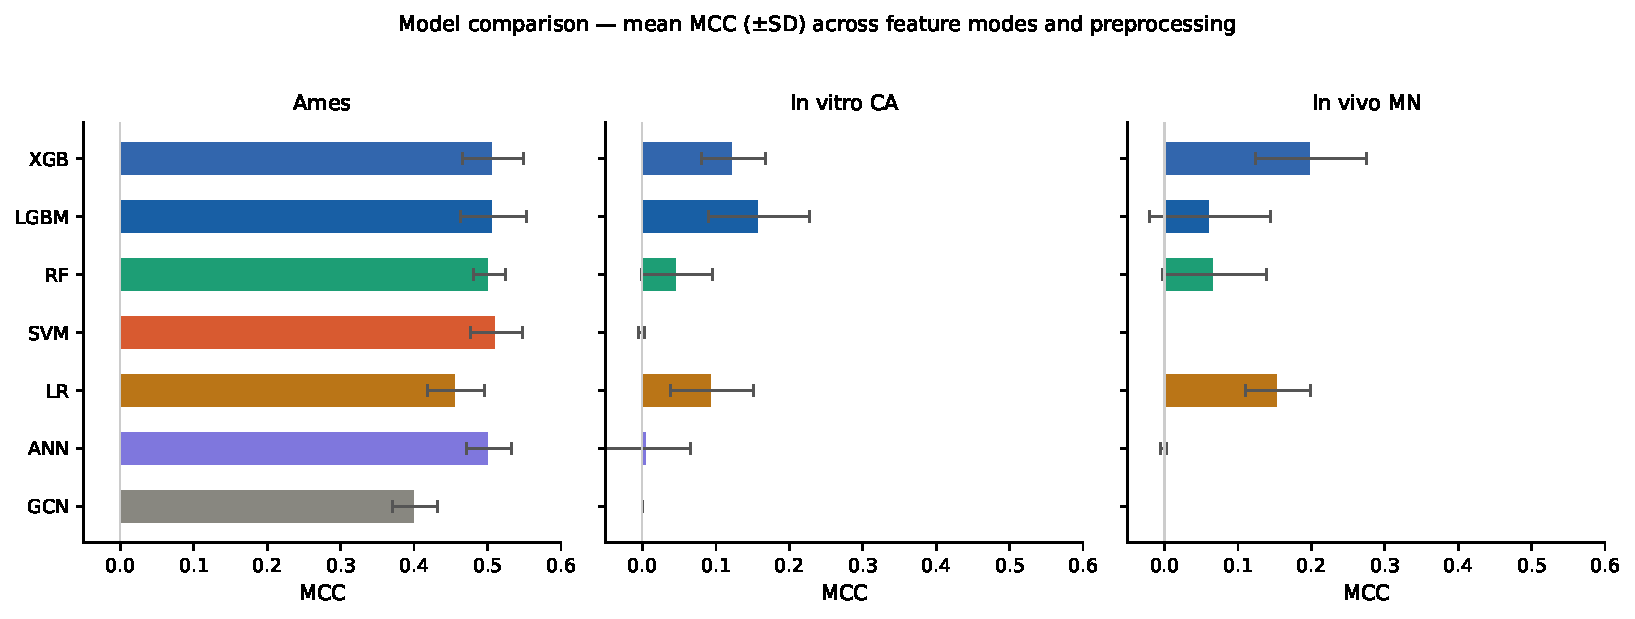
\includegraphics[width=\textwidth]{figures/figure2_model_comparison.pdf}
\caption{Mean MCC ($\pm$SD) by algorithm across all feature modes and preprocessing scenarios, grouped by endpoint.}
\label{fig:model_comparison}
\end{figure}

\subsection{Evaluation Rigor Cascade}

For Ames, random-split CV reached MCC = $0.670 \pm 0.010$, consistent with published benchmarks,\cite{Hansen_2009,Li_2021} while scaffold-split CV dropped to $0.624 \pm 0.049$ ($\Delta = 0.046$) and the held-out scaffold-split test to 0.470 (Table~\ref{tab:cascade}, Figure~\ref{fig:cascade}). Cross-source LDO produced a much larger collapse: drug $\to$ industrial reached 0.234, and industrial $\to$ drug only 0.122. The source-heterogeneity gap ($\Delta = 0.390$) was an order of magnitude larger than the split-method gap ($\Delta = 0.046$). The LDO comparison involves additional structural factors---directional asymmetry, different test sizes, and different class distributions---so $\Delta = 0.390$ is best read as a combined effect, but the magnitude difference between the two effects is unambiguous. For in~vitro CA, random and scaffold splits gave nearly identical results (0.180 vs.\ 0.189); for in~vivo MN, both values were near random given their standard deviations.

\begin{table}[ht]
\caption{Evaluation rigor cascade (locked configuration: XGBoost, compact features, raw SMILES). Level 2: mean $\pm$ SD (25 folds). Level 1: MCC [95\% bootstrap CI]. Level 3: Ames only.}
\label{tab:cascade}
\centering
\small
\begin{tabular}{@{}llccc@{}}
\toprule
Level & Evaluation method & Ames MCC & In vitro MCC & In vivo MCC \\
\midrule
2a & Random-split $5\!\times\!5$ CV & $0.670 \pm 0.010$ & $0.180 \pm 0.053$ & $0.181 \pm 0.094$ \\
2b & Scaffold-split $5\!\times\!5$ CV & $0.624 \pm 0.049$ & $0.189 \pm 0.084$ & $0.104 \pm 0.111$ \\
1 & Scaffold-split test & 0.470 [.434,.502] & 0.114 [$-$.023,.270] & 0.071 [$-$.029,.285] \\
3a & LDO: drug $\to$ industrial & 0.234 & --- & --- \\
3b & LDO: industrial $\to$ drug & 0.122 & --- & --- \\
\bottomrule
\end{tabular}
\end{table}

\begin{figure}[ht]
\centering
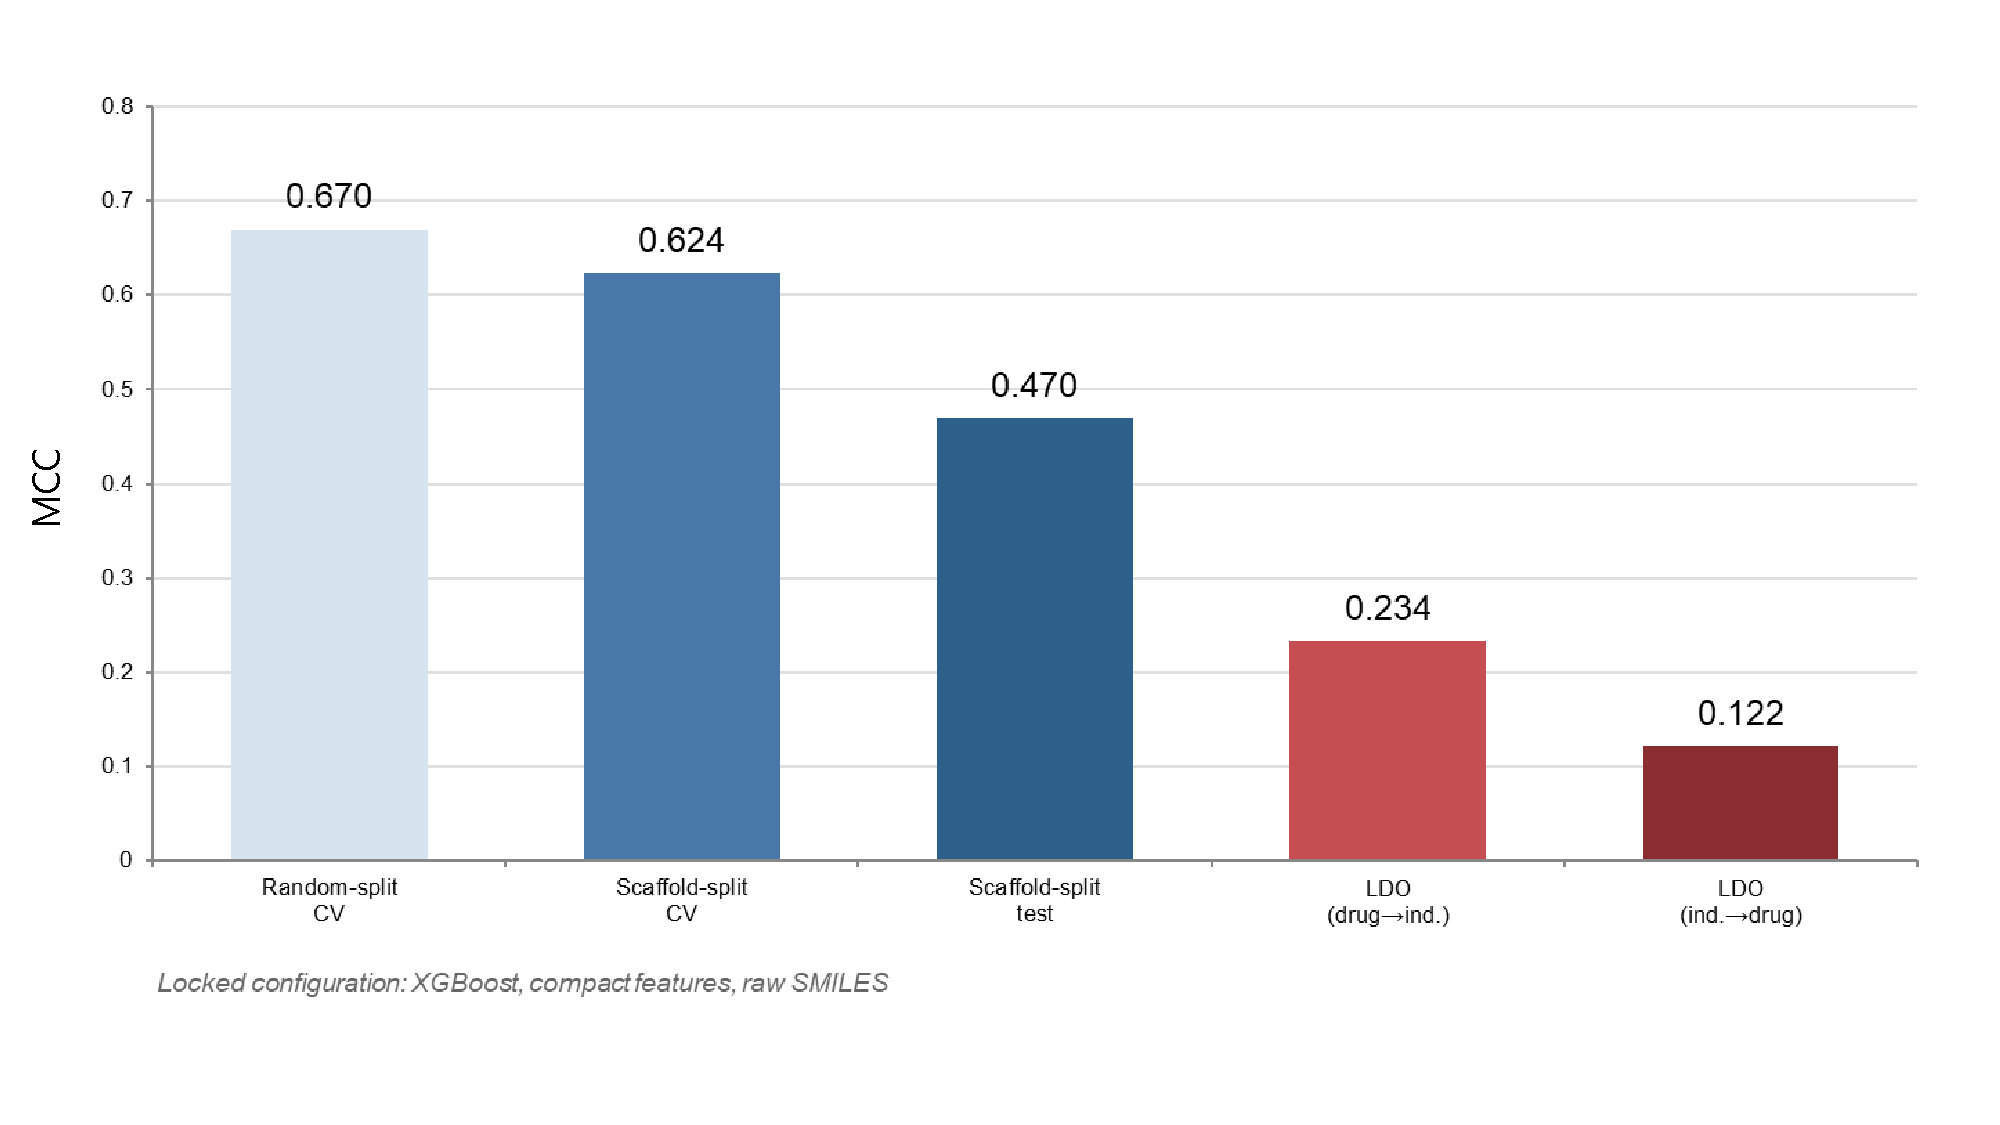
\includegraphics[width=0.85\textwidth]{figures/figure3_cascade.pdf}
\caption{Evaluation rigor cascade for Ames mutagenicity (locked configuration). The source-heterogeneity effect ($\Delta = 0.390$) substantially exceeds the split-method effect ($\Delta = 0.046$).}
\label{fig:cascade}
\end{figure}

\subsection{Source Heterogeneity and Algorithm-Specific Robustness}
\label{sec:domain}

Drug-sourced compounds ($n = 6{,}416$, positive rate 58.3\%) and industrial-sourced compounds ($n = 7{,}144$, positive rate 3.0\%) differed by a factor of 19.5 in mutagenicity prevalence (Figure~\ref{fig:domain}). A naive classifier predicting positive for drug-sourced and negative for industrial-sourced compounds achieved MCC = 0.608 and balanced accuracy = 0.834 without any structural information---comparable to the random-split CV MCC of 0.670.

LDO with three algorithms (Table~\ref{tab:ldo}) revealed two patterns. Drug $\to$ industrial generalization was uniform across algorithms (MCC 0.232--0.235). In contrast, industrial $\to$ drug exposed sharp differences: XGBoost reached only MCC = 0.122 (sensitivity 0.062), LightGBM 0.134, while Random Forest maintained MCC = 0.325 (sensitivity 0.466). We hypothesize that Random Forest's better cross-source robustness reflects feature bagging,\cite{Breiman_2001} which reduces reliance on source-correlated feature subsets.

\begin{table}[ht]
\caption{Leave-domain-out results by algorithm (Ames). Drug: $n = 6{,}416$, pos.\ rate 58.3\%. Industrial: $n = 7{,}144$, pos.\ rate 3.0\%. Naive source classifier: MCC = 0.608.}
\label{tab:ldo}
\centering
\small
\begin{tabular}{@{}lccc@{}}
\toprule
Algorithm & Drug $\to$ Ind.\ MCC & Ind.\ $\to$ Drug MCC & Ind.\ $\to$ Drug Sens. \\
\midrule
XGBoost & 0.234 & 0.122 & 0.062 \\
LightGBM & 0.232 & 0.134 & 0.081 \\
Random Forest & 0.235 & 0.325 & 0.466 \\
\bottomrule
\end{tabular}
\end{table}

\begin{figure}[ht]
\centering
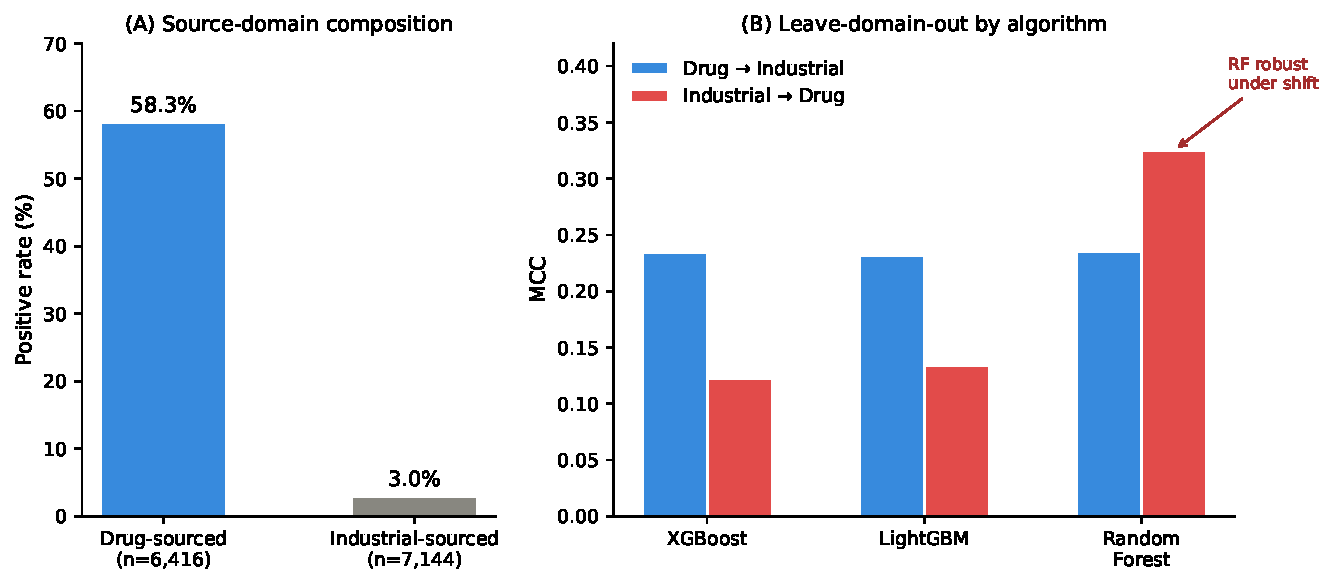
\includegraphics[width=\textwidth]{figures/figure4_domain_ldo.pdf}
\caption{Source heterogeneity in Ames. (A)~Positive rate by source: drug 58.3\% vs.\ industrial 3.0\% (19.5-fold). (B)~LDO MCC by algorithm; Random Forest is substantially more robust in the industrial$\to$drug direction.}
\label{fig:domain}
\end{figure}

\subsection{Preprocessing, In~Vivo Behavior, and Feature Importance}

\textbf{Preprocessing.} Salt stripping was strongly endpoint-specific (Figure~\ref{fig:salt}). For in~vivo MN, the best salt-stripped model reached MCC = 0.311 versus 0.086 for the best raw model ($+0.225$); salt fragments were present in 83\% of in~vivo SMILES, and among salt-containing compounds the positive rate was 2.8\% versus 7.1\% for non-salt compounds, suggesting salts were disproportionately attached to non-mutagenic compounds. For Ames, salt stripping had mixed effects ($\Delta = -0.03$ to $+0.02$); for in~vitro CA it was generally detrimental (mean MCC 0.081 $\to$ 0.056). This argues against uniform preprocessing pipelines\cite{Fourches_2010} and in favor of per-endpoint optimization.

\begin{figure}[ht]
\centering
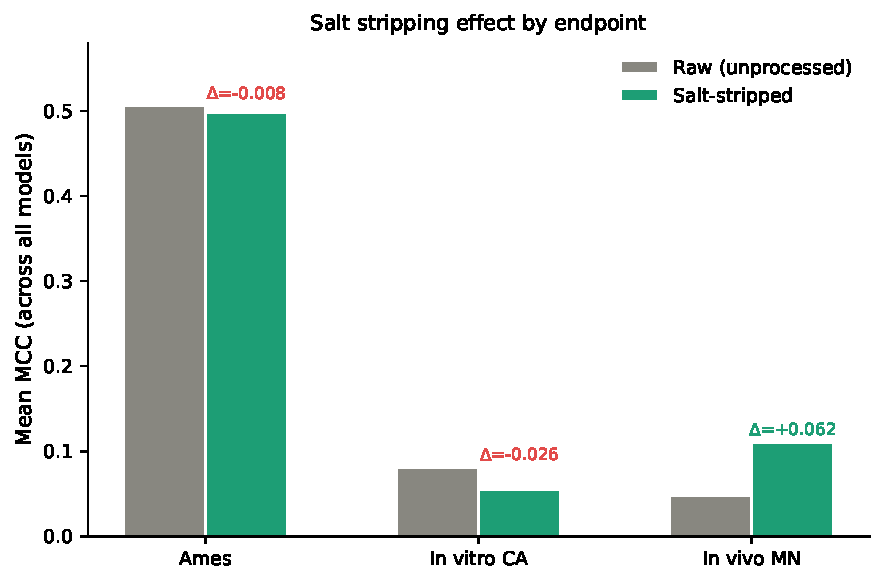
\includegraphics[width=0.75\textwidth]{figures/figure5_salt_stripping.pdf}
\caption{Effect of salt stripping on mean MCC (averaged across all models and feature modes). In~vivo improved by $+0.063$ on average and $+0.225$ for the best model; Ames mixed; in~vitro decreased.}
\label{fig:salt}
\end{figure}

\textbf{In~vivo micronucleus.} The best in~vivo model achieved ROC-AUC = 0.860 and PR-AUC = 0.237 (an 8.5-fold enrichment over the 0.028 baseline), but MCC = 0.311 with 95\% CI crossing zero ($-0.014$ to 0.571) indicates that classification at any fixed threshold is unreliable. The test set contains only 12 positives among 431 compounds. The locked-configuration learning curve was flat at MCC $\approx 0.055$ from 10\% to 100\% of training data (Figure~\ref{fig:learning_curves}), though this curve was not computed for the salt-stripped configuration.

\textbf{Feature importance.} SHAP analysis\cite{Lundberg_SHAP_2017} revealed consistent patterns (Figure~\ref{fig:shap}): physicochemical descriptors dominated the top-5 (alert count and MW for Ames; LogP for in~vitro; MW for in~vivo), and no individual fingerprint bit appeared in any top-5 list despite fingerprints comprising 50--75\% of features. Across all Ames models and scenarios, compact features yielded mean MCC = 0.448 versus 0.523 for FP-2048 ($\Delta = +0.075$), indicating that fingerprints add distributed but individually weak signal.

\begin{figure}[ht]
\centering
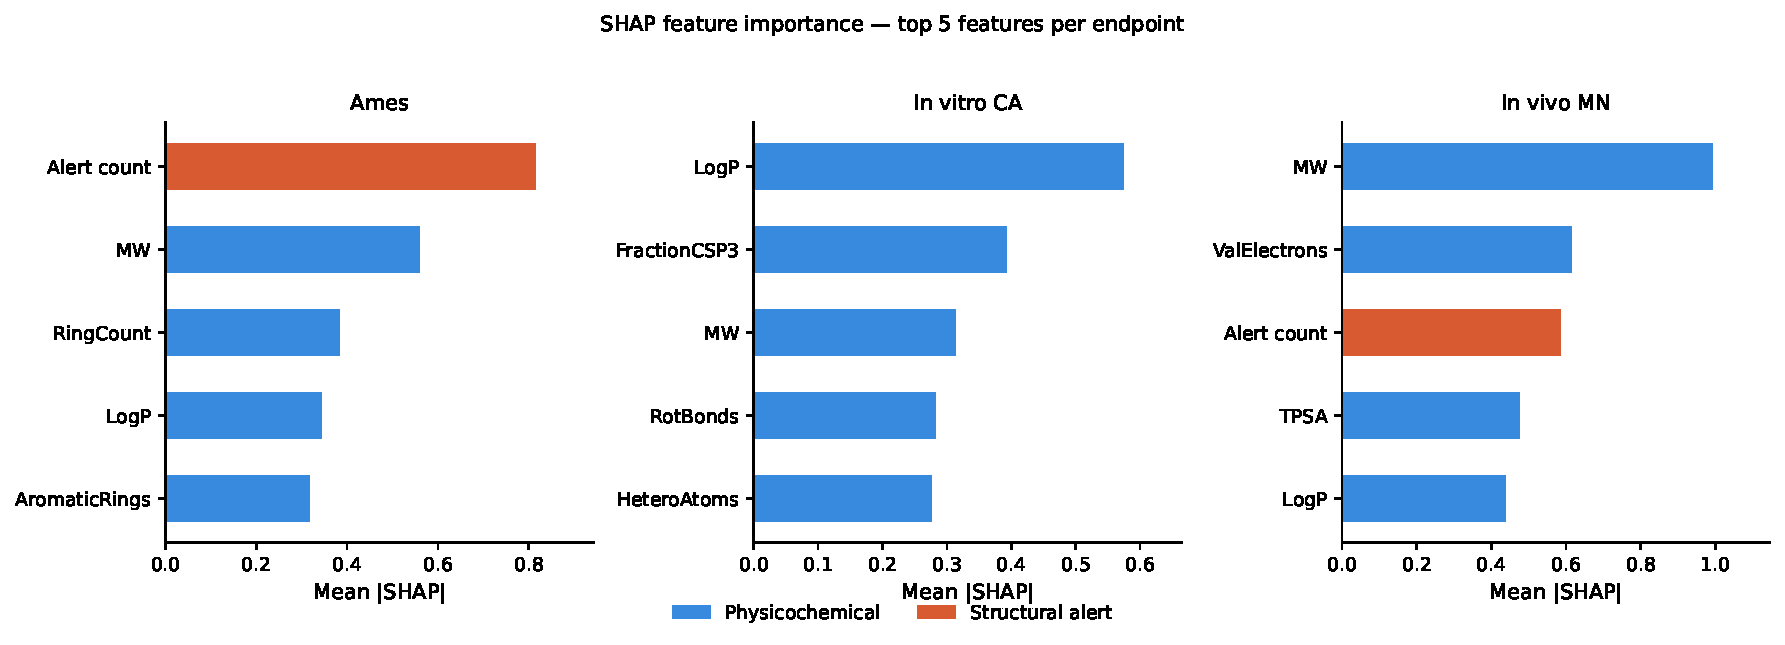
\includegraphics[width=\textwidth]{figures/figure6_shap.pdf}
\caption{SHAP top-5 features per primary endpoint. Physicochemical descriptors dominate; structural alert count ranks first for Ames. No fingerprint bits appear in any top-5.}
\label{fig:shap}
\end{figure}

\textbf{Learning curves.} Locked-configuration learning curves (Figure~\ref{fig:learning_curves}) showed three patterns: Ames MCC saturated early (0.543 at 10\%, 0.640 at 100\%); in~vitro showed a noisy upward trend ($0.070 \to 0.170$); in~vivo was flat ($\approx$0.055).

\begin{figure}[ht]
\centering
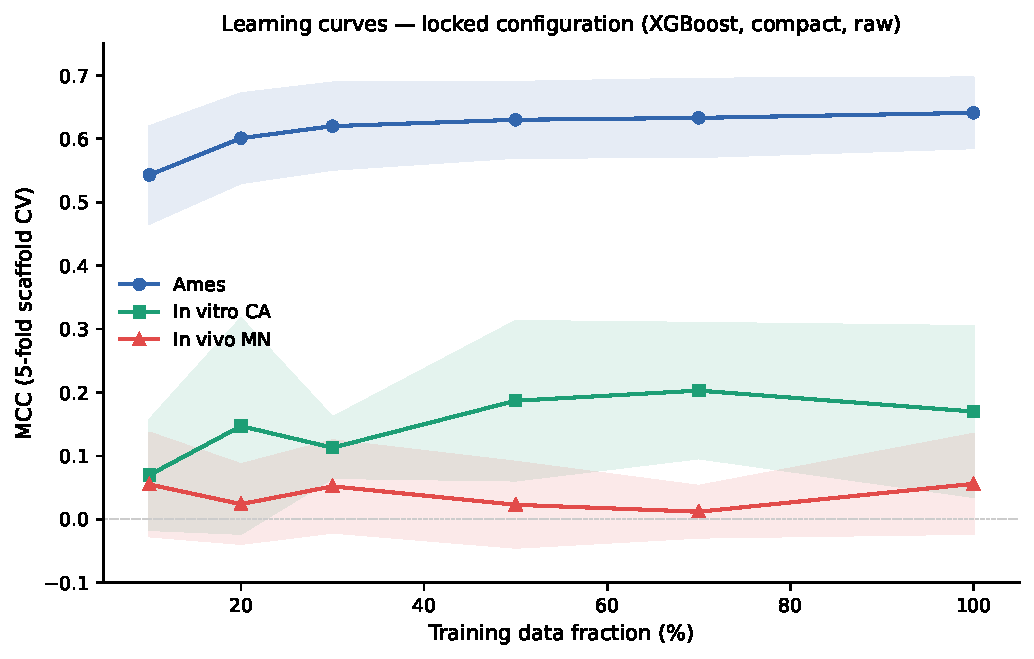
\includegraphics[width=0.8\textwidth]{figures/figure7_learning_curves.pdf}
\caption{Learning curves (locked configuration). Shaded regions: $\pm$1 SD across 5-fold scaffold CV.}
\label{fig:learning_curves}
\end{figure}
